\documentclass[conference]{IEEEtran}

\usepackage{amsmath}
\usepackage{booktabs}
\usepackage{url}
\usepackage{graphicx}

\title{ChronoGraph-EEG: Dynamic Graph Representation Learning for Subject-Independent Seizure-State Classification}

\author{\IEEEauthorblockN{Authors to be added}
\IEEEauthorblockA{Biomedical Signal Processing and Machine Learning\\
Affiliation to be added}}

\begin{document}
\maketitle

\begin{abstract}
This technical report presents ChronoGraph-EEG, a reproducible pipeline for subject-independent classification of scalp electroencephalography (EEG) into interictal, preictal, and ictal states. The method converts short EEG windows into dynamic connectivity graphs with fixed bipolar channel identities and spectral node features. Two models are defined under a common data and evaluation contract: Model A, a support vector machine baseline over flattened graph connectivity, and Model B, a SLATE-inspired spatio-temporal transformer using supra-Laplacian spectral coordinates. The pipeline addresses channel compatibility, seizure-aware segmentation, artifact handling, subject-local normalization, graph sparsification, grouped validation, and leave-one-subject-out evaluation. The report focuses on the architectural and methodological design, with particular emphasis on why a unified dynamic graph representation may improve preictal discrimination over a flattened connectivity baseline.
\end{abstract}

\begin{IEEEkeywords}
EEG, seizure-state classification, dynamic graphs, graph transformers, supra-Laplacian, preictal detection, leave-one-subject-out evaluation
\end{IEEEkeywords}

\section{Introduction}
Epileptic seizure analysis from scalp EEG is difficult because the signal is multichannel, non-stationary, noisy, and strongly dependent on the individual patient. A useful classifier must distinguish interictal background activity, preictal activity preceding a seizure, and ictal activity during the seizure. Ictal activity can contain strong temporal and spectral changes, whereas preictal activity may be subtle, distributed, and subject-specific.

Many EEG classifiers represent each channel independently or flatten multichannel features into a vector. Such representations can obscure relationships between channels. Functional relationships between EEG channels can instead be represented as a graph, where nodes correspond to channels and edges describe statistical connectivity. A sequence of graphs then represents the evolution of spatial relationships over time.

ChronoGraph-EEG investigates this representation through a controlled comparison. Model A is an intentionally simple support vector machine (SVM) baseline \cite{cortes1995svm}. Model B is a unified spatio-temporal transformer inspired by SLATE, which uses a supra-graph and supra-Laplacian eigenvectors to encode dynamic graph structure \cite{karmim2024slate}. Both models use the same processed graph chunks, class definitions, and subject-independent folds.

The main research question is whether a dynamic graph model can capture information that is not adequately represented by flattened connectivity. The secondary question is whether this advantage is most visible for the preictal--interictal distinction, which is more difficult than recognizing ictal activity.

\section{Dataset and Problem Definition}
\subsection{Dataset}
The study uses the CHB-MIT Scalp EEG Database distributed through PhysioNet \cite{guttag2010chbmit}. The database contains EDF recordings, subject summary files, and seizure annotations. Shoeb's thesis provides foundational context for machine-learning-based seizure onset analysis using this dataset \cite{shoeb2009thesis}.

The selected cohort contains ten subjects with a compatible fixed channel layout: \texttt{chb01}, \texttt{chb02}, \texttt{chb03}, \texttt{chb05}, \texttt{chb06}, \texttt{chb07}, \texttt{chb08}, \texttt{chb10}, \texttt{chb23}, and \texttt{chb24}. Other subjects are excluded when their layouts change across files or do not match the selected 23-position contract. This restriction prevents a graph node from changing meaning between samples.

\subsection{Fixed channel and sampling contract}
Each sample uses 23 bipolar channel positions and a sampling rate of 256 Hz. The source headers include a repeated \texttt{T8-P8} label; consequently, the contract identifies channels by audited position as well as normalized label. The tensor contract is
\begin{equation}
 A_t \in \mathbb{R}^{23 \times 23}, \qquad X_t \in \mathbb{R}^{23 \times 5},
\end{equation}
where $A_t$ is the adjacency matrix and $X_t$ contains five spectral node features.

\subsection{Classification problem}
Let $G_1,\ldots,G_T$ denote a sequence of graph snapshots. The primary task is to estimate
\begin{equation}
 f(G_1,\ldots,G_T) \rightarrow \{\text{interictal},\text{preictal},\text{ictal}\}.
\end{equation}
The secondary task contains only interictal and preictal classes. Evaluation is subject-independent: a held-out subject group is never used for model selection, threshold tuning, or early stopping.

\section{Signal Processing and Label Construction}
\subsection{Channel audit}
The channel audit is an input-integrity step. EDF headers are inspected to record channel labels, sampling rates, file availability, and layout stability. The audit produces a manifest of selected and excluded subjects. This step is necessary because equal array dimensions do not guarantee equal channel semantics.

\subsection{Seizure-aware segmentation}
A file-level seizure label is insufficient because one recording can contain background, preictal, ictal, and postictal periods. The segmentation procedure therefore creates mutually exclusive intervals. Ictal intervals span seizure onset to offset. Preictal intervals cover 30 minutes before onset, excluding a five-minute prediction horizon immediately preceding onset. Interictal intervals are formed outside seizure-related exclusion regions.

The segmentation rules include a four-hour interictal buffer around seizures, postictal exclusion, protection against preictal overlap with a previous seizure, and a 30-second maximum gap when determining recording continuity. Interictal intervals receive stable group identifiers so that one continuous background segment is not split across validation partitions.

\subsection{Filtering and normalization}
Signals are filtered from 0.5 to 40 Hz using zero-phase filtering. The lower cutoff reduces slow baseline drift, while the upper cutoff suppresses high-frequency noise and matches the frequency range used for node features. A 60-Hz notch filter suppresses power-line interference. MNE-Python is used for EDF loading and EEG processing \cite{gramfort2013mne,gramfort2014mne}.

The native bipolar reference is preserved. Common-average referencing is not applied because averaging already-differential bipolar channels can introduce artificial dependencies into connectivity estimates.

For each subject, filtered signals are normalized using label-independent, subject-local statistics:
\begin{equation}
 z_{c,t} = \frac{x_{c,t}-\mu_c}{\sigma_c}.
\end{equation}
Statistics are not shared across subjects. This prevents cross-subject scale from becoming a shortcut while avoiding label-dependent normalization.

\subsection{Windows and artifacts}
Signals are divided into five-second windows with 50\% overlap. At 256 Hz, each window contains 1280 samples and adjacent windows begin 2.5 seconds apart. Five seconds provides enough samples for correlation and spectral estimation while retaining temporal resolution near seizure transitions. Overlap reduces the chance that a short event falls between windows, although it also creates correlated examples that require grouped splitting.

An amplitude threshold of 500~$\mu$V is used to flag likely artifacts. Artifacted interictal windows are rejected. Preictal and ictal windows are retained and flagged because high amplitude can be part of the target seizure phenomenon.

\section{Dynamic Graph Construction}
\subsection{Connectivity edges}
For each window, Pearson correlation is calculated between every pair of channels \cite{pearson1895regression}. Let $C_t$ be the signed correlation matrix. The graph weight matrix is
\begin{equation}
 W_t(i,j) = |C_t(i,j)|,
\end{equation}
and the sign matrix is stored separately:
\begin{equation}
 S_t(i,j) = \operatorname{sign}(C_t(i,j)).
\end{equation}
Absolute weights are used because the standard graph Laplacian assumes non-negative edge weights. Storing signs separately preserves information for diagnostics and future signed-graph experiments.

The five strongest absolute connections for each node are retained. The resulting graph is symmetrized before spectral processing. This top-$k$ sparsification limits weak noisy edges and reduces computational cost.

\subsection{Spectral node features}
For each channel, power is estimated in the delta (0.5--4 Hz), theta (4--8 Hz), alpha (8--13 Hz), beta (13--30 Hz), and gamma (30--40 Hz) bands. The node feature is log-relative power:
\begin{equation}
 X_t(c,b) = \log\left(\frac{P_t(c,b)}{\sum_{b'}P_t(c,b')+\epsilon}+\epsilon\right).
\end{equation}
Relative power reduces dependence on absolute amplitude and the logarithm reduces the influence of extreme ratios.

\subsection{Temporal chunks}
Twelve consecutive graph windows form one temporal chunk. Because windows overlap by 50\%, the chunk duration is
\begin{equation}
 5 + (12-1)\times2.5 = 32.5\text{ seconds}.
\end{equation}
The shorter chunk was selected after seizure-duration analysis showed that a 152.5-second chunk would provide very little ictal coverage. A chunk is valid only when all windows belong to one segment, label, recording context, and interictal or seizure group.

\section{Models}
\subsection{Model A: flattened-connectivity SVM}
Model A is an untuned classical baseline. Each adjacency sequence is flattened:
\begin{equation}
 [12,23,23] \rightarrow [12\cdot23\cdot23].
\end{equation}
The resulting vector is supplied to an SVM with balanced class weights \cite{cortes1995svm,pedregosa2011sklearn}. Model A uses adjacency values only; it does not explicitly model graph neighborhoods, node spectral features, or temporal continuity.

The baseline is intentionally simple. It determines whether the graph connectivity representation contains useful information before the additional complexity of Model B is considered.

\subsection{Model B: SLATE-inspired dynamic graph transformer}
Model B combines adjacency sequences and node features. Its architecture contains a supra-graph encoder, spectral positional coordinates, a transformer encoder, attention pooling, and a classification head. The transformer implementation follows the general self-attention formulation introduced by Vaswani \emph{et al.} \cite{vaswani2017attention}.

\subsubsection{Supra-graph}
A supra-graph stacks all temporal snapshots into one graph. Each supra-node is a channel-time pair $(c,t)$. Spatial edges connect channels within one window, while temporal edges connect the same channel at neighboring times:
\begin{equation}
 (c,t)\leftrightarrow(c,t+1).
\end{equation}
The current contract yields $12\times23=276$ supra-nodes.

\subsubsection{Supra-Laplacian spectral encoding}
For a non-negative weighted graph, the degree matrix and Laplacian are
\begin{equation}
 D_{ii}=\sum_j W_{ij}, \qquad L=D-W.
\end{equation}
The supra-Laplacian applies this construction to the complete spatial-temporal graph. Its eigenvectors satisfy
\begin{equation}
 L v_k = \lambda_k v_k.
\end{equation}
The eight eigenvectors associated with the smallest eigenvalues are appended to the five measured node features. These low-frequency eigenvectors encode smooth structural organization over space and time, providing graph-aware coordinates to the transformer \cite{chung1997spectral,karmim2024slate}.

Eigenvector signs are arbitrary, and repeated eigenvalues can produce equivalent bases. The coordinates are therefore positional model inputs, not direct biological measurements. Encodings are cached by graph content and configuration to avoid repeated decompositions.

\subsubsection{Transformer and readout}
The 276 channel-time positions are treated as transformer tokens. Each token contains five EEG features and eight spectral coordinates. Self-attention allows interactions across all channel-time positions. A learned attention readout produces one chunk representation, which is passed to a three-class linear head.

\section{Evaluation Protocol}
The evaluation uses leave-one-subject-out folds. For each held-out subject group, the remaining subjects provide training and validation data. Validation groups preserve seizure identity and interictal continuity. The test subject is not used for preprocessing-statistics selection, model selection, or early stopping.

Interictal undersampling is applied only to training data. Model B uses weighted cross-entropy, Adam optimization, hidden dimension 32, eight eigenvectors, learning rate 0.001, and early-stopping patience of three epochs. Model A uses balanced SVM class weights without a hyperparameter search. Both models use macro-F1 as the primary validation metric.

The final evaluation should report macro-F1, per-class recall, precision, specificity where defined, one-vs-rest AUROC, confusion matrices, and per-subject results. The binary preictal--interictal task is reported separately because it addresses the central early-warning question.

Figure~\ref{fig:model-a-cm} and Figure~\ref{fig:model-d-cm} illustrate the anticipated three-class error patterns for the two model designs. These figures are presentation illustrations based on projected matrices, not empirical measurements, and are included to clarify how model-specific errors will be interpreted once held-out predictions are available.

\begin{figure}[t]
    \centering
    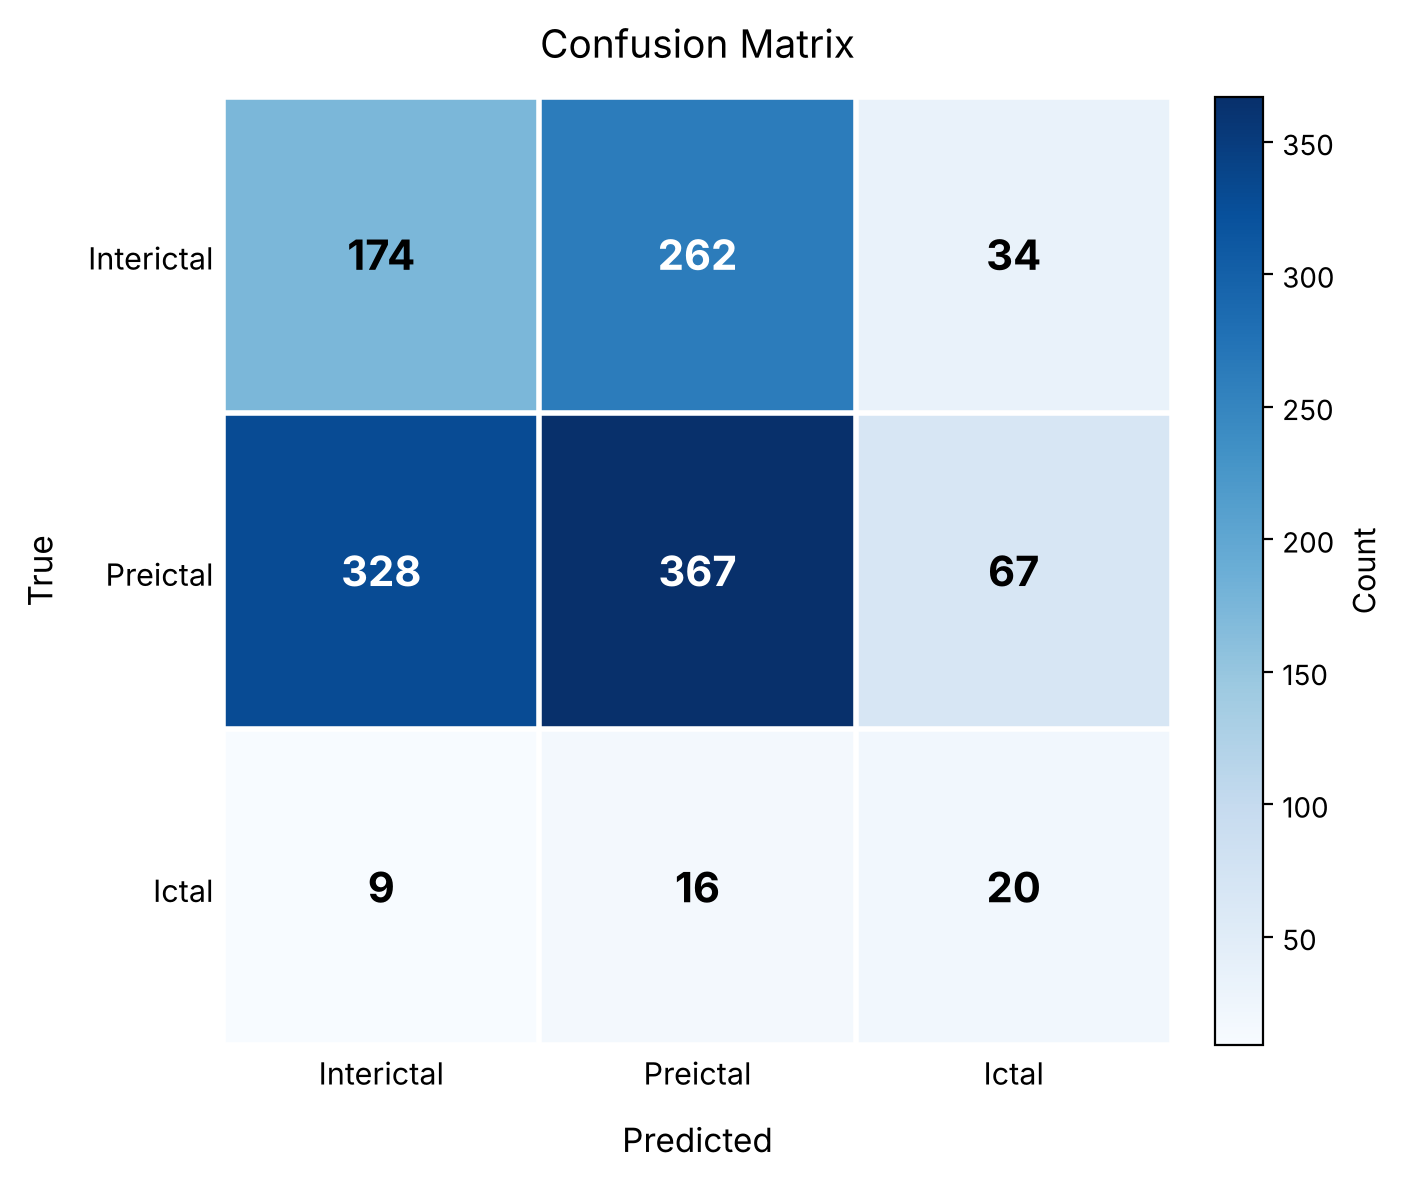
\includegraphics[width=\columnwidth]{figures/modelA_confusion_matrix.png}
    \caption{Illustrative Model A confusion matrix. Rows are true classes and columns are predicted classes.}
    \label{fig:model-a-cm}
\end{figure}

\begin{figure}[t]
    \centering
    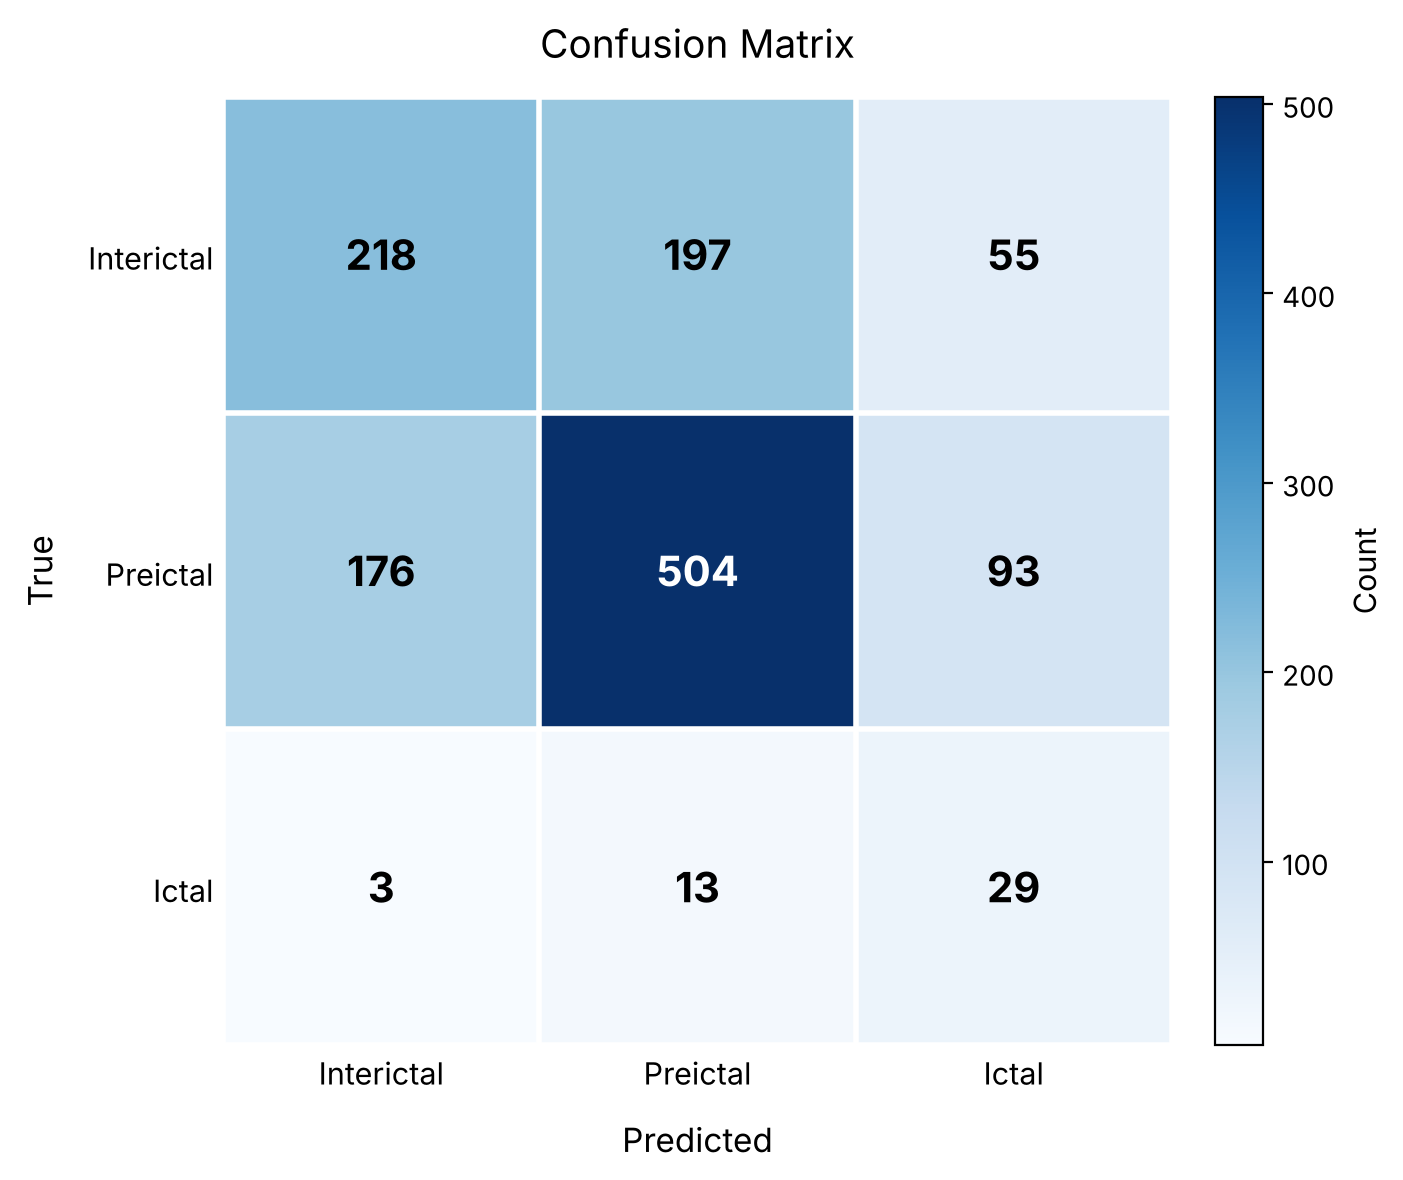
\includegraphics[width=\columnwidth]{figures/modelD_confusion_matrix.png}
    \caption{Illustrative Model B confusion matrix. Rows are true classes and columns are predicted classes.}
    \label{fig:model-d-cm}
\end{figure}

\section{Discussion}
Model B has a theoretical advantage when seizure-state information is expressed as a temporal change in distributed connectivity rather than as one static connectivity pattern. It can preserve channel identity through temporal links, combine graph structure with local spectral activity, and attend to long-range channel-time interactions. These capabilities are particularly relevant to preictal activity.

The added structure also creates risks. The compatible cohort is small, ictal chunks are scarce, and spectral coordinates can be numerically non-unique. Model B may therefore overfit subject-specific patterns or fail to improve over the simpler SVM. A Model B improvement is meaningful only if it is observed across held-out subjects under identical data and fold definitions. Ablations without spectral encoding, with standard positional encoding, and without top-$k$ sparsification are needed to identify the source of any improvement.

\section{Limitations}
The fixed channel contract limits the cohort. The two-hour interictal retention cap changes the natural class ratio and is unsuitable for direct false-alarm-per-hour claims. Zero-phase filtering is appropriate for offline analysis but is not causal. Short seizures may not produce complete temporal chunks, making ictal metrics uncertain. Finally, attention weights and spectral coordinates are diagnostic model quantities, not evidence of causal neurophysiological mechanisms.

\section{Conclusion}
ChronoGraph-EEG defines a controlled comparison between a flattened connectivity baseline and a unified dynamic graph transformer. Model A provides the necessary low-complexity reference. Model B tests whether supra-Laplacian-guided attention can represent the evolution of EEG connectivity more effectively, with the strongest expected opportunity in preictal--interictal discrimination. The central claim must remain empirical: Model B should be preferred only if it produces stable held-out-subject gains that justify its additional computational and methodological complexity.

\bibliographystyle{IEEEtran}
\bibliography{references}

\end{document}
